\documentclass[sigplan,screen]{acmart}

%%
%% \BibTeX command to typeset BibTeX logo in the docs
\AtBeginDocument{%
	\providecommand\BibTeX{{%
Bib\TeX}}}

\usepackage{emoji}
\usepackage{applekeys}

% \setemojifont{Apple Color Emoji}

\begin{document}

\title{GNU, Free software and Stallman's dedication}
\keywords{GNU, Free Software, they made me put this keywords section}

\author{Stan Ioan-Victor 832}
\email{ioan.victor.stan@stud.ubbcluj.ro}

\begin{teaserfigure}
	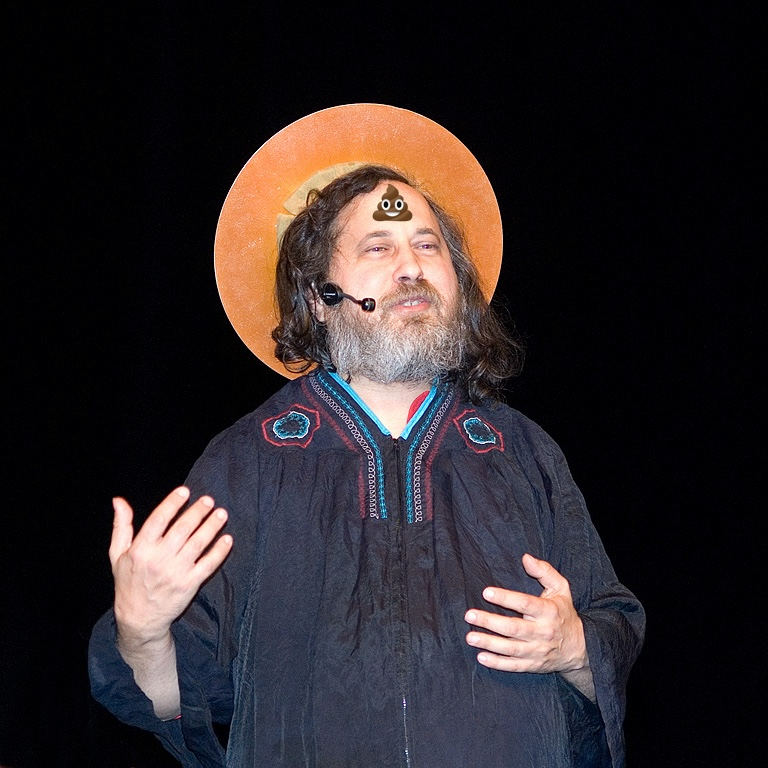
\includegraphics[width=200px]{pics/jesus-stallman.jpg}
	\centering
	\caption{RMS, Chief GNUisance in his divine prime}
	\Description{Stallman, in costume as St. IGNUcius, wearing a halo consisting of the platter of an old hard disk drive (Monastir, Tunisia, 2012); description provided by Wikipedia, but picture slighly vandalised by me, adding a poop emoji on his forehead for reasons discussed towards the latter of the essay}
	\label{fig:teaser}
\end{teaserfigure}

%% This command processes the author and affiliation and title
%% information and builds the first part of the formatted document.
\maketitle

One of (I feel like) most important key aspects that often goes overlooked in today's "SIGN UP HERE, SUBSCRIBE THERE, ACCEPT MY COOKIESS PlsPLSPLPS" age is privacy and freedom of your personal data or just having technology DO WHAT YOU NEED/WANT IT TO, where now \href{https://www.youtube.com/watch?v=MPyJBJTHyO0}{Facebook requires 1384 hoola hoops}\cite{tantacrul} through which you need to jump just to exercise your right to be forgotten, and where \href{https://www.youtube.com/watch?v=LZzubS1ILTs}{Microsoft shoves ads down your throat}\cite{jakey} when you use their bloated Windows "file search" \textbf{dis-service}\cite{BarraDRM} that forces your prompt through Bing. It's such a shame because these computing things are amazing, they just got handcuffs on them.

But this guy, \textbf{up above} was concerned we might come to this before there even was any code highlighting.

\textbf{Richard Matthew Stallman} (rms) was right in a way, since his cautionary tale all the way back from '97: \href{https://www.gnu.org/philosophy/right-to-read.html}{The Right to Read}\cite{Stallman1997TheRT} has become kind of true over the past years, when services that you technically don't own get re-branded as "products"\cite{product}, but they could rug-pull you at any moment, everything from film\cite{jellyfin}, to of course, as the previous citations pointed out, literature and education.

So how did we get here, and when did my mans realize a change is needed?

\section{That damn symbolics.com}
In the early 80's, Stallman was working on his lil version of the Lisp interpreter, when software conglomerate \href{https://symbolics.com}{symbolics} asked if they could use it for a bit (will give it back unworn promise ongong fr \emoji{crossed-fingers}). You see, Symbolics is a manufacturer of exactly \ldots \textbf{ Lisp machines}, which are exactly what they sound like.

What's important about them is: they are, believe it or not, actually so OG, they were the veryy first \textbf{domain name} ever registered on the internet in 1985. Wayy before ICANN was even a thing and they had to shake hands with "the National Science Foundation (NSF)". ICANN only came out in '95. \cite{national-science-foundation}

Now since Stallman accepted to give them the interpreter via a \textbf{public domain} lisence, they had no qualms about modifying it and keeping it in-house. He then tried to ask for those mods back but he never got them.

His grudge was so intense after that incident that he decided to start the

\section{Free software movement}
In '83 rms launched an OS that would be like Unix, in the sense of its impact and user experience, but not in the sense of how locked-down it was to modifications and its proprietary nature, Unix being owned by AT\&T primarily. He came up with the genious (\verb|\s|) recursive acrnonym of \textbf{G}NU's not Unix. Cuz it wasn't\ldots Unix. "GNU" was so damn good they even named an asteriod after it. \cite{gnu-asteriod}

He basically set out to "free" Unix.

The philosophy behind "free" is the main point of contention for a lot of people learning about the free software movement.

The term broadly reffers to:

\begin{quote}
	"
	software that comes with permission for anyone to use, copy, and/or distribute, either verbatim or with modifications, either gratis or for a fee.
	"
\end{quote}

in their words, putting it best:
\begin{quote}
	"
	you should think of "free" as in "free speech," not as in "free beer."
	"
\end{quote}

Meaning there are 4 \textbf{essential} freedoms the users of such programs benefit from: \label{freedoms}
\begin{quotation}
	\begin{itemize}
		\item 	The freedom to run the program as you wish, for any purpose. (freedom 0)
		\item 	The freedom to study how the program works, and change it so it does your computing as you wish. Access to the source code is a precondition for this. (freedom 1)
		\item  	The freedom to redistribute copies so you can help others. (freedom 2)
		\item  	The freedom to distribute copies of your modified versions to others. By doing this you can give the whole community a chance to benefit from your changes. Access to the source code is a precondition for this. (freedom 3)
	\end{itemize}
\end{quotation}

Now, armed with the belief that this is the only ethical form of making / distributing software, rms founded the \textbf{Free Software Foundation} (FSF) in 1985, accepting donations and support of even technical kind, in building one of the most important software library in history. Not neccesarily because they initially set out to build them, but because that's what was needed to have a complete, free system. \cite{gnu-and-linux}

You might've heard about a few projects from that library, both end-user focused:
\begin{itemize}
	\item GIMP (\href{https://www.youtube.com/watch?v=pVI_smLgTY0}{pewd's ally now}) \cite{pewds-linux}
	\item LibreOffice (the brokies know)
	\item emacs (most comprehensive OS)
	\item GNOME (for beautiful UI's)\cite{gnome}
\end{itemize}
And developer-useful
\begin{itemize}
	\item The GNU Compiler Collection (GCC)
	\item GNU Binutils (things like the linker, assembler etc.)
	\item flex
	\item bison
	\item gdb
	\item gscript
	\item BASHHH!! bro, bash
\end{itemize}
And all of these user-space tools were fantastic and sysadmins everywhere were replacing their proprietary counterparts, but the only problem was that they had to be run on top of a non-free kernel and operating system, and they had to be boostrapped by them, usually Unix. They didn't quitee make up a "complete" system just yet.

So they started working on HURD, GNU's free kernel, so they could once and for all distance themselves from non-free software forever. \cite{hurd}

But before they could get it working, one faithful January day in 1992, \textbf{Linus Benedict Torvalds} (yes, like the eggs) put out the release notes for Linux v0.12, his \href{https://www.gnu.org/philosophy/words-to-avoid.en.html#Freemium}{gratis} Kernel, on which he's been working since 1991 (might'a heard of it, no biggie)\cite{linux-init-release-note}, stating:
\begin{quote}
	… I propose that the
	copyright be changed so that it confirms to GNU …
\end{quote}\cite{linux-becomes-free}

\ldots

MONUMENTAL!!!, this is the moment this iconic, out-of-a-superhero-cereal-box figure was created:
\begin{figure}[H]
	\centering
	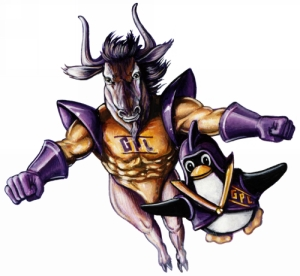
\includegraphics[width=\columnwidth]{pics/gnu-and-penguin.jpg}
	\Description{Picture of GNU's mascot (a wildebeest) flying alongide Linux's mascot (a pengiun)}
	\caption{a GNU and a lil pengu}
	\label{fig:gnu-linux}
\end{figure}
And so, GNU/Linux "or as I've recently taken to calling it, GNU plus Linux." \cite{gnu-and-linux} was created.

I was thinking of writing more about their distinction and the beef rms has with words and terminology, but I'll instead just leave these references here. \cite{gnu-vs-linux-1} \cite{gnu-vs-linux-2} \cite{gnu-vs-linux-3} Hopefully this won't be needed because you now know the history, but \verb|tl;dr| is: in terms of source-code proportions — GNU makes up more of a GNU / Linux distribution than the Linux part. I mean Linus literally used the GNU toolset to build the kernel, so yeah ... in a way it's a biproduct itself now.

Also more recent versions of Linux have come with binary modules, some considering it not as free. But just to make it clear, it's still "open-source" just not free. Yeah, they're different things, not confusing at all: \cite{free-vs-open-source}

Now what all of these programs had in common was a \textbf{free} license, not necessarily the in-house produced GNU General Public License, but others that abbided by the aforementioned 4 freedoms \ref{freedoms}. Some include Apache, MIT, BSD, zlib.

\href{https://www.gnu.org/philosophy/categories.html}{Cool breakdown here}. \cite{free-categories}

This doesn't mean there can't be ANY restrictions when distributing modified versions.

In fact, even the copy of the original, \\
free \verb|sample-sigplan.tex| file distributed by ACM that I used for this \TeX   double-column format had the requirement of

\begin{quote}
	"
	Any modified versions of this file must be renamed
 with new filenames distinct from \verb|sample-sigplan.tex|
	"
\end{quote}
and
\begin{quote}
	"
	This generated file may be distributed as long as the
 original source files, as listed above, are part of the
 same distribution.
	"
\end{quote}
What does the FSF have to say about this?
\begin{quote}
	"
	This sort of requirement is acceptable only if there's a suitable aliasing facility that allows you to specify the original program's name as an alias for the modified version.
	"
\end{quote}
And I mean … I only ever had to change the name of \textbf{this} file and everything else just snapped into place, so checks out.

So the FSF is not only a collective of developers working to make this a reality, but also a legal team focused on protecting the rights and freedom imposed by free software.

They imploy a \textbf{copyleft}\textsuperscript{\textcopyleft} framework on top of their \textbf{copy right-ed}\textsuperscript{\textcopyright} work to enforce freedoms (\ref{freedoms}), essentially relaxing copyright. At the beggening of their journey, legal disputes weren't handled too formally, but instead just through regular, email exchanges between rms + FSF's lawyer, Eben Moglen and whoever was causing trouble in paradise. It was usually people trying to close down software intially distributed through GPL, not including the original GPL with the re-distributed software, as required by the license, for example.

They could even represent \textbf{you} in court. \cite{about-gnu}

\section{The pivotal point}
In 2003, a Cisco subsidiary, wifi-routers producing company \textbf{Linksys} broke GPL by shipping their devices with compiled firmware derived from free software, without including the modified sources and licence, like GPL states you need to do, hence "stealing" free software. \cite{fsf-vs-cisco}

FSF ended up suing and eventually Cisco followed suit, even appointing a Free Software Director for Linksys and even donated a bit to FSF. This demonstrated the FSF's willingness to use legal action to enforce the GPL against a major corporation. \cite{cisco-lawsuit-start} \cite{cisco-lawsuit-end}

Since before, people were confused on how that would even work. \cite{linksys-legend}

\par

Other conglomerates were also found breaking such rights, including Microsoft using GPLv2 code for a device boot tool. \cite{microsoft-steal-gpl} Eventually complying to it and releasing the tool along with the source-code as well.

OpenTV, Motorola, Acer, Panasonic, and even Orange were kinda under scrutiny for simmillar practices. \cite{orange-naughty}

Not even farmers are safe from this, \textbf{John Deere} is using free software in their tractors but are not letting their users study, modify and repair them in case anything goes wrong, requiring them to come back to ol' John for repairs. \cite{john-deere} This kinda reminds me of the right to repair
Louis Rossmann was boasting about. \cite{rossman-right-to-repair}

All-in-all, what they're trying their best to build is an inclusive community of hackers and users, just trying to do some computing.

Yeahh, all of their websites have this old-timey feeling to it, just plain HTML and eye-piercing whitemode: \href{https://www.gnu.org}{gnu.org}, \href{https://www.fsf.org}{fsf.org}, \href{https://www.stallman.org}{stallman.org} (good thing OperaGX has one of the best "force dark-mode" features out there)
but it's kinda charming in that sense as well. To be honest, the most important information you'll find is usually on websites looking like that.

One thing I've noticed, though the "marketing" for GNOME is kind of better, which makes sense, considering that it's a UI: \href{https://www.gnome.org}{gnome.org}

And they're also trying to bring the trend to the masses thorugh "it's ok if you're not a guru, we can install it for you" campaigns: \href{https://endof10.org/places/}{endof10.org}. Omg that rhymed, I didn't even notice, I should be part of their campaigns.

They're also really really back-wards compatible with everything they try to do. For god's sake they only discontinued official physical-disk support for copies of \TeX-Live last year \ldots BUT YOU CAN STILL PERSONALLY ASK somebody from TUG to burn a DVD for you:: \cite{texlive-on-dvd}

\section{I'm broke, and you're asking me to be broker?}
Nah man, you \textbf{can} make money from developing / maintaining / distributing free software, as confusing as that sounds, but they explain more about free, Commercial software \href{https://www.gnu.org/philosophy/categories.en.html}{here}. \cite{free-categories}

And you don't have to work on just donations, like
\href{https://godotengine.org}{Godot} and \href{https://www.blender.org}{Blender}, but can offer paid software consultancy like \href{https://deeproot.in}{DeepRoot GNU/Linux} does for free infra., or could even do it for your own free programs, after all, the best that know the program is those who made it! You'd be getting paid for your active time, not just the product itself. Or just costimizations like \href{https://cfc.net.in}{Computing Freedom Collective} does. If you heard about PureOS, you might like to know that its development is sponsored by selling liberty-respecting hardware \href{https://puri.sm}{puri.sm}. You can also sell free programs to people intending to use them in proprietary scenarios: \href{https://www.gnu.org/philosophy/selling-exceptions.html}{Selling exceptions}. \href{https://www.redhat.com/en/technologies/linux-platforms/enterprise-linux}{RedHat} is also doing \href{https://cs.stanford.edu/people/eroberts/cs201/projects/open-source/econ.htm}{not to bad}.

But essentially, yeah you're restricting yourself a ton if you roll like rms and refuse to use non-free programs as of today, maybe come back in 15 years.

His dedication to this, though is pretty insane and doesn't care about convenience. He goes as far as not having a mobile phone … at all, not a dumb one, just none. Only paying in cash no matter what, old-school taxis, NEVER SHOW ID. Not owning an Intel CPU made after 2006, and AMD's simmilarly. Only got a burner credit card for buying flight tickets and car-rentals. Always disables Javascript on all websites, especially obfuscated one. If you wanna invite him for a conference and you can't have your registration website run without JS, sorry, he ain't coming. Also, PEPSI > COCA-COLA obv (this is actually heavier than it sounds).
\cite{stallman-paranoid-1} \cite{stallman-paranoid-2} \cite{dont-use-intel}

\section{Ok but he said \ldots}
Yeah, tbh rms {\huge \textbf{is}} a weirdo with statements like: (\textbf{obvious \textcolor{red}{trigger warning} please don't ruin your day}): \cite{bro-wtf-1} \cite{bro-wtf-2} \cite{bro-wtf-3} \cite{bro-wtf-4} \cite{bro-wtf-5} \cite{bro-wtf-toate}
Which got me confused about how auto-contrary the 2 definitions of "symposium" is
\begin{figure}[H]
	\centering
	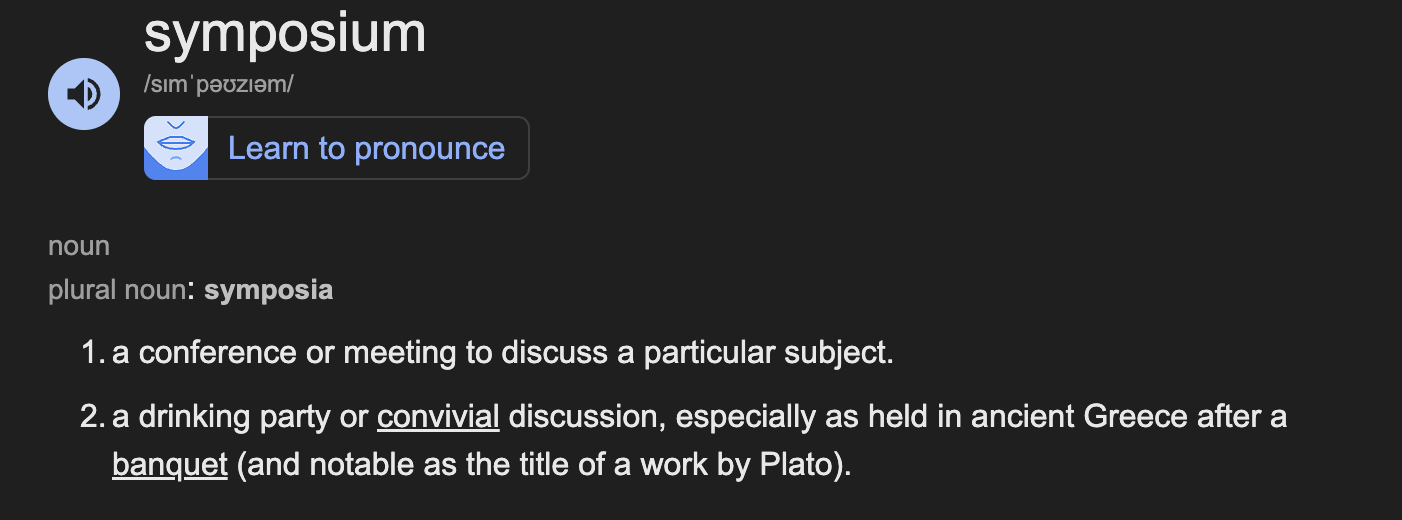
\includegraphics[width=\columnwidth]{pics/symposium.png}	
	\Description{Definition of the word symposium. 1. A conference / meeting (formal); 2. A drinking party (a bit less formal if you could call it that)}
	\label{fig:symposium-def}
\end{figure}
If you know, you know, and if you don't, it's honestly better that way cuz I don't wanna poison your mind.

Yeah, maybe don't write life-long essays with everything that pops into your head (much like this one felt). I just wouldn't wanna be seen walking around with him, but sure, I'll compile my C++ in GCC.

I didn't even know about these before I started researching and writing this essay, tbh now I regret putting up a big picture of him in a crown as the teaser \ldots Maybe vandalising it will make me feel better.

UPDATE : Didn't help that much

\section{The community tho}
Even though he might be dead to some people now after those things, the legacy he left behind is still here, and FSF recently celebrated 40 years of GNU. Believe it or not, there actually are a ton of other real-people behind it. \cite{gnu-forty-years}
\begin{figure}[H]
	\includegraphics[width=\columnwidth]{pics/gnu40-deani.jpg}	
	\caption{Ppl at the 40th anniversary in Biel/Bienne, 2023.}
	\Description{Picture of people at the 40-th anniversary of GNU in Biel/Bienne, 2023.}
	\label{fig:gnu-anniversary}	
\end{figure}
Ok, I know rms was also there. \cite{gnu-forty-years-stallman}

These people still keep the proliferation of free software alive, which is hypocritical of me to say considering I'm currently typing on a keyword that has the keys \cmdkey \ctlkey \optkey, and most importantly: \applekey    on it.

Other than that thanks a ton for readingg and I hope you didn't fall asleep more than twice!!

\bibliographystyle{ACM-Reference-Format}
\bibliography{biblio}

%% If your work has an appendix, this is the place to put it.
% \appendix

\end{document}
\endinput